%===============================================================
% ABC Music Suite 技術文書
% メインファイル
% コンパイル: latexmk -pdfdvi main.tex
%           または: platex main && dvipdfmx main
%===============================================================
\documentclass[a4paper,11pt]{jlreq}

%---------------------------------------------------------------
% パッケージ
%---------------------------------------------------------------
\usepackage[dvipdfmx]{graphicx,xcolor}
\usepackage{tikz}
\usetikzlibrary{
  shapes.geometric, arrows.meta, positioning, fit,
  decorations.pathreplacing, calc, backgrounds,
  shadows.blur, matrix, chains, trees
}
\usepackage{pgfplots}
\pgfplotsset{compat=1.18}
\usepackage{float}               % [H]の位置指定用

\usepackage{listings}            % ソースコード
\usepackage{tcolorbox}           % カラーボックス
\tcbuselibrary{listings,skins,breakable,theorems}
\usepackage{booktabs}            % 美しい表
\usepackage{tabularx}
\usepackage{longtable}
\usepackage{multirow}
\usepackage{enumitem}
\usepackage{geometry}
\usepackage[dvipdfmx]{hyperref}
\usepackage{fancyhdr}            % ヘッダ・フッタ
\usepackage{titlesec}            % セクション見出し
\usepackage{mdframed}
\usepackage{amsmath}
\usepackage{fontawesome5}        % アイコン（要 fontawesome5 パッケージ）
\usepackage{pifont}
\usepackage{array}
\usepackage{dirtree}             % ディレクトリツリー

%---------------------------------------------------------------
% ページレイアウト
%---------------------------------------------------------------
\geometry{
  top=25mm, bottom=25mm,
  left=25mm, right=25mm,
  headheight=29pt
}
\addtolength{\topmargin}{-14pt}

%---------------------------------------------------------------
% カラーパレット（システムのデザインに合わせたダークブランドカラー）
%---------------------------------------------------------------
\definecolor{brand-cyan}{RGB}{34,211,238}
\definecolor{brand-purple}{RGB}{124,58,237}
\definecolor{brand-green}{RGB}{74,222,128}
\definecolor{brand-blue}{RGB}{96,165,250}
\definecolor{bg-dark}{RGB}{11,17,32}
\definecolor{bg-card}{RGB}{20,30,50}
\definecolor{text-muted}{RGB}{148,163,184}
\definecolor{accent-red}{RGB}{248,113,113}
\definecolor{node-api}{RGB}{34,211,238}
\definecolor{node-midi}{RGB}{74,222,128}
\definecolor{node-ollama}{RGB}{167,139,250}
\definecolor{node-ui}{RGB}{96,165,250}
\definecolor{node-rpi}{RGB}{251,191,36}
\definecolor{codebg}{RGB}{15,23,42}

%---------------------------------------------------------------
% セクション見出しスタイル
%---------------------------------------------------------------
\titleformat{\section}
  {\Large\bfseries\color{brand-purple}}
  {\thesection}{1em}{}[{\color{brand-cyan}\titlerule[1.5pt]}]

\titleformat{\subsection}
  {\large\bfseries\color{brand-cyan!80!black}}
  {\thesubsection}{1em}{}

\titleformat{\subsubsection}
  {\normalsize\bfseries\color{brand-purple!70!black}}
  {\thesubsubsection}{1em}{}

%---------------------------------------------------------------
% ソースコードスタイル
%---------------------------------------------------------------
\lstset{
  basicstyle=\ttfamily\small\color{white},
  keywordstyle=\color{brand-cyan}\bfseries,
  commentstyle=\color{text-muted}\itshape,
  stringstyle=\color{brand-green},
  numbers=left,
  numberstyle=\tiny\color{text-muted},
  numbersep=8pt,
  frame=single,
  rulecolor=\color{brand-purple!40},
  backgroundcolor=\color{codebg},
  breaklines=true,
  breakatwhitespace=true,
  showstringspaces=false,
  tabsize=4,
  extendedchars=false
}

% Python用
\lstdefinestyle{python}{
  language=Python,
  morekeywords={async,await,def,class,return,import,from,with}
}

% PowerShell用
\lstdefinestyle{powershell}{
  language=bash,
  morekeywords={Write-Host,Start-Process,Set-Location,Test-Path,Copy-Item}
}

% ABC記法用
\lstdefinestyle{abc}{
  language={},
  basicstyle=\ttfamily\small\color{brand-green},
  backgroundcolor=\color{codebg},
}

%---------------------------------------------------------------
% tcolorboxスタイル
%---------------------------------------------------------------
\tcbset{
  mybox/.style={
    enhanced,
    colback=bg-card,
    colframe=brand-purple!60,
    fonttitle=\bfseries\color{white},
    coltitle=white,
    coltext=white,
    attach boxed title to top left={yshift=-2mm,xshift=4mm},
    boxed title style={
      colback=brand-purple,
      colframe=brand-purple,
      rounded corners
    }
  },
  tipbox/.style={
    enhanced,
    colback=brand-cyan!8,
    colframe=brand-cyan!60,
    leftrule=4pt,
    sharp corners=west
  },
  warnbox/.style={
    enhanced,
    colback=accent-red!8,
    colframe=accent-red!60,
    leftrule=4pt,
    sharp corners=west
  },
  notebox/.style={
    enhanced,
    colback=brand-green!8,
    colframe=brand-green!60,
    leftrule=4pt,
    sharp corners=west
  }
}

%---------------------------------------------------------------
% ヘッダ・フッタ
%---------------------------------------------------------------
\pagestyle{fancy}
\fancyhf{}
\fancyhead[L]{\small\color{text-muted}ABC Music Suite --- 技術文書}
\fancyhead[R]{\small\color{text-muted}\rightmark}
\fancyfoot[C]{\small\color{text-muted}\thepage}
\renewcommand{\headrulewidth}{0.4pt}
\renewcommand{\headrule}{\hbox to\headwidth{\color{brand-purple!40}\leaders\hrule height \headrulewidth\hfill}}

%---------------------------------------------------------------
% ハイパーリンク
%---------------------------------------------------------------
\hypersetup{
  colorlinks=true,
  linkcolor=brand-purple,
  urlcolor=brand-cyan,
  citecolor=brand-green,
  pdftitle={ABC Music Suite 技術文書},
  pdfauthor={情報科学演習},
  pdfsubject={ローカルLLM × 音楽生成システム}
}

%---------------------------------------------------------------
% 便利コマンド
%---------------------------------------------------------------
\newcommand{\api}[1]{\texttt{\color{brand-cyan}#1}}
\newcommand{\file}[1]{\texttt{\color{brand-green}#1}}
\newcommand{\cmd}[1]{\texttt{\color{brand-purple}#1}}
\newcommand{\port}[1]{\textbf{\color{brand-cyan}:#1}}
\newcommand{\okmark}{\textcolor{brand-green}{\ding{52}}}
\newcommand{\ngmark}{\textcolor{accent-red}{\ding{56}}}

%===============================================================
% ドキュメント本文
%===============================================================
\begin{document}

%---------------------------------------------------------------
% タイトルページ
%---------------------------------------------------------------
\begin{titlepage}
  \begin{tikzpicture}[remember picture, overlay]
    % 背景グラデーション風
    \fill[bg-dark] (current page.south west) rectangle (current page.north east);
    % 装飾円
    \fill[brand-purple, opacity=0.15]
      (current page.north west) + (3,-3) circle (6cm);
    \fill[brand-cyan, opacity=0.10]
      (current page.south east) + (-4,4) circle (5cm);
    \fill[brand-purple, opacity=0.08]
      (current page.center) + (0,2) circle (8cm);
    % 上部ライン
    \draw[brand-cyan, line width=2pt]
      (current page.north west) + (2,-2) --
      (current page.north east) + (-2,-2);
    % 下部ライン
    \draw[brand-purple, line width=2pt]
      (current page.south west) + (2,2) --
      (current page.south east) + (-2,2);
  \end{tikzpicture}

  \vspace*{3cm}
  \begin{center}
    {\fontsize{14}{18}\selectfont\color{brand-cyan}\texttt{ローカルLLM × 音楽生成システム}}\\[1em]
    {\fontsize{40}{50}\selectfont\bfseries\color{white}ABC Music}\\[0.3em]
    {\fontsize{40}{50}\selectfont\bfseries\color{brand-cyan}Suite}\\[0.5em]
    {\color{brand-purple!70!white}\rule{12cm}{1.5pt}}\\[1.5em]
    {\fontsize{16}{20}\selectfont\color{white}\bfseries 技術文書 v2.0}\\[0.8em]
    {\color{text-muted}\large システム設計・構成・API仕様・セットアップガイド}\\[3cm]

    
\begin{tikzpicture}
      \node[draw=brand-cyan, line width=1pt, rounded corners=8pt,
            fill=bg-card, text=white,
            minimum width=8cm, minimum height=1.5cm, font=\large\bfseries] {
        ♪ \quad ABC Music Suite \quad ♪
      };
    \end{tikzpicture}

    \vfill
    {\color{text-muted}
      情報科学演習 \quad $|$ \quad
      2026年6月 \quad $|$ \quad
      Powered by Ollama (ローカルLLM)
    }
  \end{center}
\end{titlepage}

%---------------------------------------------------------------
% 目次
%---------------------------------------------------------------
{
  \color{brand-purple!30}
  \renewcommand{\contentsname}{目次}
  \tableofcontents
}
\newpage

%===============================================================
%===============================================================
% 01_overview.tex - システム概要
%===============================================================
\section{システム概要}

\file{ABC Music Suite}は、ローカルマシン上で動作する大規模言語モデル（LLM）である「Ollama」を活用し、音楽の自動作曲、ハーモニー（伴奏）の付与、および楽譜・音源データの変換と管理を一元的に行うことができる統合システムです。

外部のクラウドAPIキー（ChatGPTやClaudeなど）を一切必要とせず、すべてのAI推論プロセスがローカル環境で完結するため、機密性の高いオフライン環境や、通信帯域に制限のある環境（Raspberry Piなど）でも安定して動作します。

\subsection{主な機能}

本システムは、音楽制作とAIインタラクションをサポートする5つのコア機能を提供します。それぞれの機能の詳細は表\ref{tab:system_functions}の通りです。

\begin{table}[htbp]
  \centering
  \caption{ABC Music Suiteの主要機能一覧}
  \label{tab:system_functions}
  \begin{tabularx}{\textwidth}{p{4cm} X}
    \toprule
    \textbf{機能名} & \textbf{説明} \\
    \midrule
    \textbf{\faMagic\ 自動作曲} & ユーザーが入力したテーマ（例：「爽やかな朝の森」）や音楽的パラメータ（キー、テンポ）に基づいて、AIがABC記法の楽譜を自動生成し、即座にMIDIおよびWAV音声としてレンダリング・再生します。 \\
    \addlinespace
    \textbf{\faMusic\ ハーモニー付与} & 単旋律（メロディのみ）のABC楽譜に対して、AIが自動的に適切な伴奏コード（和音）や追加のパートを構成し、ハーモニー豊かな楽曲へとアップグレードします。 \\
    \addlinespace
    \textbf{MIDI $\leftrightarrow$ ABC変換} & 既存のMIDIファイルをテキストベースのABC記法に、またはその逆に変換します。変換エンジンには、定評あるオープンソースの \cmd{abc2midi} および \cmd{midi2abc} を使用し、高い互換性を実現しています。 \\
    \addlinespace
    \textbf{\faComments\ AIチャット} & Ollama上のローカルLLMと自由に対話できるチャットUIを提供します。会話中にAIがABC記法で音楽コードを出力した場合、システムが自動的にそれを検出し、Web画面上で即座に楽譜表示および演奏できるようにします。 \\
    \addlinespace
    \textbf{\faLaptopCode\ Raspberry Pi連携} & 同一ローカルネットワーク（LAN）上に存在するRaspberry Piから、PC上の強力なOllamaサーバーに接続し、コマンドラインベースでAIチャットや自動演奏を実行します。 \\
    \bottomrule
  \end{tabularx}
\end{table}

\begin{tcolorbox}[notebox, title=ローカルファーストのメリット]
  本システムはローカルLLM（デフォルトでは \texttt{qwen3.5:9b} を推奨）をベースに設計されています。
  これにより、インターネット接続が不要となり、APIの利用料金や利用制限を気にすることなく、無限に音楽の作成・実験を行うことができます。また、PCに搭載されたGPU（NVIDIA製GeForceなど）を最大限に活用することで、数秒〜十数秒での高速な楽譜生成が可能です。
\end{tcolorbox}

%===============================================================
% 02_architecture.tex - システム構成・アーキテクチャ
%===============================================================
\section{システムアーキテクチャ}

本システムは、機能ごとの責務を明確に分離した「マルチレイヤー（多層）アーキテクチャ」を採用しています。各コンポーネント間は疎結合に設計されており、API（HTTP/SSE）および明確なインターフェースを介してのみ通信を行います。

\subsection{全体システム構成図}

システム全体の構造および各サブシステムの通信関係を図\ref{fig:overall_arch}に示します。

\begin{figure}[H]
  \centering
  \begin{tikzpicture}[
    scale=0.75, every node/.style={transform shape},
    node distance=1.6cm and 2.2cm,
    % スタイル定義
    subsys/.style={draw=brand-purple!60, fill=bg-card!5, dashed, rounded corners=8pt, inner sep=12pt, font=\small\bfseries},
    node-ui/.style={draw=node-ui, fill=node-ui!10, rounded corners=4pt, minimum width=3.2cm, minimum height=0.8cm, align=center, font=\small\bfseries},
    node-api/.style={draw=node-api, fill=node-api!10, rounded corners=4pt, minimum width=3.2cm, minimum height=0.8cm, align=center, font=\small\bfseries},
    node-midi/.style={draw=node-midi, fill=node-midi!10, rounded corners=4pt, minimum width=3.2cm, minimum height=0.8cm, align=center, font=\small\bfseries},
    node-ollama/.style={draw=node-ollama, fill=node-ollama!10, rounded corners=4pt, minimum width=3.2cm, minimum height=0.8cm, align=center, font=\small\bfseries},
    node-rpi/.style={draw=node-rpi, fill=node-rpi!10, rounded corners=4pt, minimum width=3.2cm, minimum height=0.8cm, align=center, font=\small\bfseries},
    link/.style={-{Latex[length=8pt]}, thick, draw=brand-purple!80},
    dlink/.style={{Latex[length=8pt]}-{Latex[length=8pt]}, thick, draw=brand-cyan!80, dashed}
  ]

  % Subgraph: Browser
  \node[node-ui] (ui) {Vite + React UI};
  \node[node-ui, below=0.3cm of ui] (tabs) {Compose / Harmonize\\MidiConvert / Chat};
  \node[draw=node-ui!50, dotted, rounded corners=6pt, fit=(ui) (tabs), label={[node-ui]above:Webブラウザ (\port{5173})}] (browser) {};

  % Subgraph: FastAPI
  \node[node-api, right=3.5cm of ui] (fastapi) {FastAPI (main.py)};
  \node[node-api, below=0.3cm of fastapi] (routes) {routes/ (各APIルーター)};
  \node[node-api, below=0.3cm of routes] (llmclient) {modules/llm\_client.py};
  \node[node-api, below=0.3cm of llmclient] (synthesizer) {abc\_synthesizer.py};
  \node[draw=node-api!50, dotted, rounded corners=6pt, fit=(fastapi) (routes) (llmclient) (synthesizer), label={[node-api]above:FastAPIバックエンド (\port{8000})}] (python-server) {};

  % Subgraph: Node.js
  \node[node-midi, right=3.5cm of fastapi] (express) {Express (server.js)};
  \node[node-midi, below=0.4cm of express] (abc2midi) {abc2midi.exe};
  \node[draw=node-midi!50, dotted, rounded corners=6pt, fit=(express) (abc2midi), label={[node-midi]above:MIDIサーバー (\port{3001})}] (node-server) {};

  % Subgraph: Ollama
  \node[node-ollama, below=1.2cm of python-server] (ollama) {Ollama API};
  \node[node-ollama, below=0.3cm of ollama] (models) {qwen3.5 / qwen2.5};
  \node[draw=node-ollama!50, dotted, rounded corners=6pt, fit=(ollama) (models), label={[node-ollama]below:Ollama LLMサーバー (\port{11434})}] (ollama-server) {};

  % Subgraph: Raspberry Pi
  \node[node-rpi, left=3.5cm of ollama-server] (rpi-play) {play\_abc.py (演奏)};
  \node[node-rpi, below=0.3cm of rpi-play] (rpi-synth) {abc\_synthesizer.py (合成)};
  \node[draw=node-rpi!50, dotted, rounded corners=6pt, fit=(rpi-play) (rpi-synth), label={[node-rpi]below:Raspberry Pi (音声再生デバイス)}] (rpi) {};

  % コネクション
  \draw[link] (tabs.east) -- node[above, text=brand-purple, font=\tiny\bfseries] {HTTP POST / SSE} (routes.west);
  \draw[link] (express.west) -- node[above, text=brand-cyan, font=\tiny\bfseries] {Proxy} (fastapi.east);
  \draw[link] (express.south) -- (abc2midi.north);
  \draw[link] (llmclient.south) -- node[left, text=brand-purple, font=\tiny\bfseries] {HTTP REST} (ollama.north);
  \draw[link] (rpi-play.south) -- (rpi-synth.north);
  \draw[link] (routes.south) -- (llmclient.north);
  \draw[link] (routes.south) -- (synthesizer.north);

\end{tikzpicture}
\caption{ABC Music Suite システムアーキテクチャ全体図}
\label{fig:overall_arch}
\end{figure}

\subsection{ポート割り当て一覧}

システム各コンポーネントが占有するネットワークポートおよび通信プロトコルの一覧を表\ref{tab:ports}に示します。

\begin{table}[htbp]
  \centering
  \caption{サービスポート一覧}
  \label{tab:ports}
  \begin{tabularx}{\textwidth}{l l l X}
    \toprule
    \textbf{サービス名} & \textbf{標準ポート} & \textbf{プロトコル} & \textbf{役割} \\
    \midrule
    \textbf{Vite Dev Server} & \port{5173} & HTTP & フロントエンド(React)の開発用Web配信 \\
    \textbf{FastAPI Backend} & \port{8000} & HTTP / SSE & メインAPIサービス、ファイル配信、SSEストリーミング \\
    \textbf{MIDI Server} & \port{3001} & HTTP & abc2midi / midi2abc ラッパープロキシ \\
    \textbf{Ollama Service} & \port{11434} & HTTP & ローカルLLM推論API \\
    \bottomrule
  \end{tabularx}
\end{table}

\subsection{主要データフロー}

システムの動作時におけるデータの流れをシーケンス図形式で示します。

\subsubsection{自動作曲シーケンス}

ユーザーがWeb UIから曲のテーマを入力して作曲を指示した際、バックエンドで楽譜テキストが抽出され、音声波形（WAV）として合成されるまでの流れを図\ref{seq:compose}に示します。

\begin{figure}[H]
  \centering
  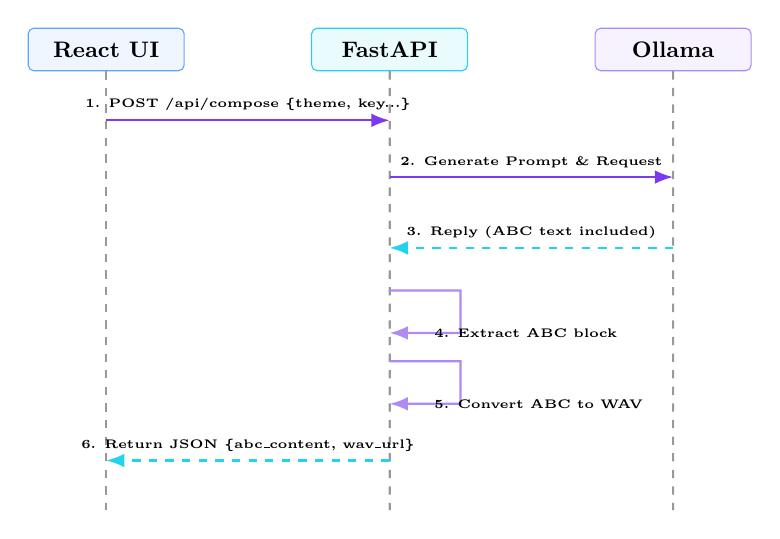
\begin{tikzpicture}[
    scale=0.9, every node/.style={transform shape},
    lifeline/.style={draw, dashed, gray!80, thick},
    node-ui/.style={draw=node-ui, fill=node-ui!10, rounded corners=2pt, font=\small\bfseries, minimum width=2.2cm, minimum height=0.6cm},
    node-api/.style={draw=node-api, fill=node-api!10, rounded corners=2pt, font=\small\bfseries, minimum width=2.2cm, minimum height=0.6cm},
    node-ollama/.style={draw=node-ollama, fill=node-ollama!10, rounded corners=2pt, font=\small\bfseries, minimum width=2.2cm, minimum height=0.6cm},
    msg/.style={-Latex, thick, draw=brand-purple},
    reply/.style={-Latex, thick, dashed, draw=brand-cyan},
    self-msg/.style={-Latex, thick, draw=brand-purple!60}
  ]

  % ライフラインヘッダ
  \node[node-ui] (ui) at (0,0) {React UI};
  \node[node-api] (api) at (4,0) {FastAPI};
  \node[node-ollama] (ol) at (8,0) {Ollama};

  % ライフライン縦線
  \draw[lifeline] (ui.south) -- (0,-6.5);
  \draw[lifeline] (api.south) -- (4,-6.5);
  \draw[lifeline] (ol.south) -- (8,-6.5);

  % メッセージの描画
  \draw[msg] (0,-1) -- node[above, font=\tiny\bfseries] {1. POST /api/compose \{theme, key...\}} (4,-1);
  \draw[msg] (4,-1.8) -- node[above, font=\tiny\bfseries] {2. Generate Prompt \& Request} (8,-1.8);
  \draw[reply] (8,-2.8) -- node[above, font=\tiny\bfseries] {3. Reply (ABC text included)} (4,-2.8);

  % 自己呼び出し (FastAPI内の処理)
  \draw[self-msg] (4,-3.4) -- ++(1,0) -- ++(0,-0.6) -- node[right, pos=0.5, font=\tiny\bfseries] {4. Extract ABC block} (4,-4.0);
  \draw[self-msg] (4,-4.4) -- ++(1,0) -- ++(0,-0.6) -- node[right, pos=0.5, font=\tiny\bfseries] {5. Convert ABC to WAV} (4,-5.0);

  \draw[reply] (4,-5.8) -- node[above, font=\tiny\bfseries] {6. Return JSON \{abc\_content, wav\_url\}} (0,-5.8);

\end{tikzpicture}
\caption{自動作曲処理のデータフロー}
\label{seq:compose}
\end{figure}

\subsubsection{MIDI・ABC相互変換シーケンス}

MIDIファイルが入力され、Node.js Expressに配置された外部実行バイナリ \file{abc2midi} 等を経由して変換が実行されるフローを図\ref{seq:midi_convert}に示します。

\begin{figure}[H]
  \centering
  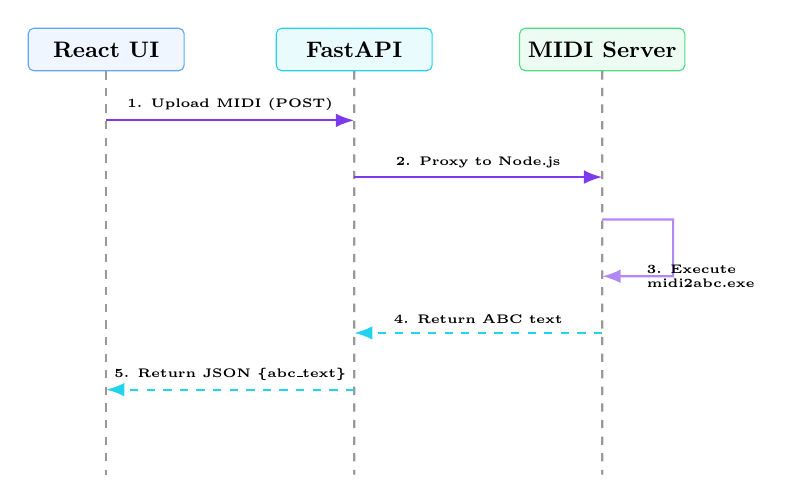
\begin{tikzpicture}[
    scale=0.9, every node/.style={transform shape},
    lifeline/.style={draw, dashed, gray!80, thick},
    node-ui/.style={draw=node-ui, fill=node-ui!10, rounded corners=2pt, font=\small\bfseries, minimum width=2.2cm, minimum height=0.6cm},
    node-api/.style={draw=node-api, fill=node-api!10, rounded corners=2pt, font=\small\bfseries, minimum width=2.2cm, minimum height=0.6cm},
    node-midi/.style={draw=node-midi, fill=node-midi!10, rounded corners=2pt, font=\small\bfseries, minimum width=2.2cm, minimum height=0.6cm},
    msg/.style={-Latex, thick, draw=brand-purple},
    reply/.style={-Latex, thick, dashed, draw=brand-cyan},
    self-msg/.style={-Latex, thick, draw=brand-purple!60}
  ]

  % ライフラインヘッダ
  \node[node-ui] (ui) at (0,0) {React UI};
  \node[node-api] (api) at (3.5,0) {FastAPI};
  \node[node-midi] (node) at (7,0) {MIDI Server};

  % ライフライン縦線
  \draw[lifeline] (ui.south) -- (0,-6);
  \draw[lifeline] (api.south) -- (3.5,-6);
  \draw[lifeline] (node.south) -- (7,-6);

  % メッセージ
  \draw[msg] (0,-1) -- node[above, font=\tiny\bfseries] {1. Upload MIDI (POST)} (3.5,-1);
  \draw[msg] (3.5,-1.8) -- node[above, font=\tiny\bfseries] {2. Proxy to Node.js} (7,-1.8);

  % 自己呼び出し (Node.jsから外部バイナリ実行)
  \draw[self-msg] (7,-2.4) -- ++(1,0) -- ++(0,-0.8) -- node[right, pos=0.5, font=\tiny\bfseries, align=left] {3. Execute\\midi2abc.exe} (7,-3.2);

  \draw[reply] (7,-4.0) -- node[above, font=\tiny\bfseries] {4. Return ABC text} (3.5,-4.0);
  \draw[reply] (3.5,-4.8) -- node[above, font=\tiny\bfseries] {5. Return JSON \{abc\_text\}} (0,-4.8);

\end{tikzpicture}
\caption{MIDIからABCへの変換フロー}
\label{seq:midi_convert}
\end{figure}

%===============================================================
% 03_setup.tex - 環境構築・セットアップ
%===============================================================
\section{環境構築とセットアップ}

本システムは、Windows 10/11 をホストPCとし、LAN経由でRaspberry Piなどの外部デバイスと接続することを想定しています。以下にシステムを稼働させるためのセットアップ手順を説明します。

\subsection{前提条件・必要環境}

本システムを実行するには、ホストPCに以下のソフトウェアがあらかじめインストールされている必要があります。

\begin{itemize}
  \item \textbf{Ollama}: ローカルで大規模言語モデルを実行するエンジン。
    \begin{itemize}
      \item 推奨モデル: \texttt{qwen3.5:9b} または \texttt{qwen2.5-coder:7b}（音楽記法（ABC記法）の生成において高い安定性を示します）。
    \end{itemize}
  \item \textbf{Python 3.10以上}: バックエンドの FastAPI サーバー動作に必要。
  \item \textbf{Node.js 18以上}: フロントエンドの開発・ビルドおよび MIDI サーバー動作に必要。
\end{itemize}

\subsection{依存関係のインストール}

リポジトリをクローンまたは展開した後、各ディレクトリで必要なパッケージをインストールします。

\subsubsection{1. Python バックエンドの依存関係}
コマンドプロンプトまたは PowerShell を起動し、以下のコマンドを実行します。
\textbf{Pythonバックエンドの依存パッケージインストール:}\\
\begin{lstlisting}[style=powershell]
cd C:\情報科学演習\server
pip install fastapi uvicorn pydantic requests
\end{lstlisting}

\subsubsection{2. Node.js MIDI サーバーの依存関係}
MIDIファイルの相互変換およびラッパーとして動作するExpressサーバーの依存関係をインストールします。
\textbf{Node.js MIDIサーバーの依存パッケージインストール:}\\
\begin{lstlisting}[style=powershell]
cd C:\情報科学演習\midi-server
npm install
\end{lstlisting}

\subsubsection{3. フロントエンド (React) の依存関係}
Vite + React ベースの Web UI 用パッケージをインストールします。
\textbf{フロントエンドの依存パッケージインストール:}\\
\begin{lstlisting}[style=powershell]
cd C:\情報科学演習\web-ui
npm install
\end{lstlisting}

\subsection{起動手順}

\subsubsection{一括起動 (推奨)}
本システムには、フロントエンド、バックエンド、MIDIサーバーの3つのサービスを一括で立ち上げるスクリプトが用意されています。

PowerShell から起動する場合は、以下のコマンドを実行します。
\textbf{PowerShellによる一括起動コマンド:}\\
\begin{lstlisting}[style=powershell]
cd C:\情報科学演習
.\start.ps1
\end{lstlisting}

また、エクスプローラーから \file{start.bat} をダブルクリックすることでも、同様にすべてのサービスを一括起動できます。

\subsubsection{個別起動 (開発・デバッグ用)}
サービスを個別にデバッグしたい場合は、3つのターミナルを開き、それぞれ以下のコマンドを実行します。

\begin{enumerate}
  \item \textbf{FastAPI バックエンド}:
    \begin{lstlisting}[style=powershell]
cd C:\情報科学演習\server
python -m uvicorn main:app --host 127.0.0.1 --port 8000 --reload
    \end{lstlisting}
  \item \textbf{MIDI サーバー}:
    \begin{lstlisting}[style=powershell]
cd C:\情報科学演習\midi-server
node server.js
    \end{lstlisting}
  \item \textbf{Web UI (Vite)}:
    \begin{lstlisting}[style=powershell]
cd C:\情報科学演習\web-ui
npm run dev
    \end{lstlisting}
\end{enumerate}

\subsection{起動後のアクセス先URL}

すべてのサービスが正常に起動すると、表\ref{tab:endpoints}のURLから各サービスにアクセスできます。

\begin{table}[htbp]
  \centering
  \caption{アクセス先URL一覧}
  \label{tab:endpoints}
  \begin{tabularx}{\textwidth}{l l X}
    \toprule
    \textbf{アクセス先} & \textbf{URL} & \textbf{説明} \\
    \midrule
    \textbf{Web UI} & \url{http://localhost:5173} & \textbf{メインの操作画面（ここをブラウザで開きます）} \\
    \textbf{FastAPI Swagger} & \url{http://localhost:8000/docs} & バックエンドのAPI仕様確認・テスト用インタラクティブ画面 \\
    \textbf{FastAPI API} & \url{http://localhost:8000} & フロントエンドやラズパイからアクセスされるAPIベース \\
    \textbf{MIDI Server} & \url{http://localhost:3001} & MIDI変換を処理するNode.jsのエンドポイント \\
    \bottomrule
  \end{tabularx}
\end{table}

\subsection{設定の変更}

\subsubsection{OllamaサーバーのIPアドレス設定}
デフォルトでは、FastAPIは同一マシン上のOllama（\url{http://127.0.0.1:11434}）に接続します。
Raspberry Piなど他のデバイスから接続する場合、またはOllamaを別PCで動かす場合は、\file{server/modules/config.py} を編集します。

\textbf{config.py の編集例:}\\
\begin{lstlisting}[style=python]
# Set Ollama server IP
OLLAMA_HOST = "192.168.0.136"  # Change to your host PC's IP address
OLLAMA_PORT = 11434
\end{lstlisting}

また、環境変数 \texttt{OLLAMA\_HOST} を設定することでも上書き可能です。
\begin{lstlisting}[style=powershell]
$env:OLLAMA_HOST = "192.168.0.136"
.\start.ps1
\end{lstlisting}

%===============================================================
% 04_usage.tex - システムの利用方法
%===============================================================
\section{システムの利用方法}

サービスを一括起動した後、ブラウザで \url{http://localhost:5173} を開くと、統合Web UIが表示されます。UIは上部のタブで切り替えることができ、それぞれの機能を提供します。

また、UIの右上には「接続ステータスインジケーター」があり、OllamaサーバーおよびMIDIサーバーへの接続状態がリアルタイムで緑（接続中）または赤（切断）で表示されます。

\subsection{\texorpdfstring{\faMagic\ 自動作曲タブ}{自動作曲タブ}}

AIに指示を出して完全に新しい楽曲を生成させることができます。

\begin{enumerate}
  \item \textbf{テーマの入力}: 「爽やかな朝」「哀愁漂う夜の街」など、曲のイメージをテキストで自由に入力します。
  \item \textbf{パラメータ設定}:
    \begin{itemize}
      \item \textbf{キー（調号）}: C, G, F, Am, Em などから選択します。
      \item \textbf{テンポ（BPM）}: 60〜200 の範囲で設定します。
    \end{itemize}
  \item \textbf{使用モデルの選択}: ドロップダウンから、Ollamaにロードされている任意のLLMモデル（例: \texttt{qwen3.5:9b}）を選択します。
  \item \textbf{実行}: 「作曲を開始」ボタンをクリックします。
  \item \textbf{結果の確認}: 数秒後、AIが生成した楽譜テキスト（ABC記法）とレンダリングされた楽譜が画面に表示されます。また、画面上のオーディオプレーヤーで生成された音源（WAV）をその場で再生でき、ダウンロードも可能です。
\end{enumerate}

\subsection{\texorpdfstring{\faMusic\ ハーモニー付与タブ}{ハーモニー付与タブ}}

既存の単旋律（メロディのみ）に対して、AIに伴奏（コードまたは別パート）を追加させることができます。

\begin{enumerate}
  \item \textbf{メロディ入力}: テキストエリアに既存のABC記法の楽譜を貼り付けます。
  \item \textbf{モデルと設定の選択}: 自動作曲と同様に、モデルを設定します。
  \item \textbf{実行}: 「ハーモニーを生成」ボタンをクリックします。
  \item \textbf{結果の確認}: メロディラインに伴奏（コードや低音パートなど）が追加された新しい楽譜が生成されます。同様に、オーディオプレーヤーで和音を伴った演奏の再生・ダウンロードが可能です。
\end{enumerate}

\subsection{\texorpdfstring{MIDI $\leftrightarrow$ ABC変換タブ}{MIDI-ABC変換タブ}}

PC上のMIDIファイルとテキストベースのABC楽譜を双方向に変換できます。

\begin{figure}[htbp]
  \centering
  \begin{tcolorbox}[mybox, title={MIDI $\leftrightarrow$ ABC 双方向変換の操作}]
    \textbf{■ MIDIからABCへ変換する手順}
    \begin{enumerate}
      \item ファイル選択エリアで、PC内にある \file{.mid} ファイルをドラッグ＆ドロップまたはクリックして選択します。
      \item 「ABCへ変換」ボタンをクリックします。
      \item 変換後のABC楽譜テキストが表示され、画面上で楽譜のプレビューおよび音源再生ができます。
    \end{enumerate}
    \vspace{0.2cm}
    \textbf{■ ABCからMIDIへ変換する手順}
    \begin{enumerate}
      \item エディタエリアに、直接ABC記法のテキストを入力または貼り付けます。
      \item 「MIDIへ変換」ボタンをクリックします。
      \item 変換に成功すると、生成された \file{.mid} ファイルのダウンロードリンクが表示されます。
    \end{enumerate}
  \end{tcolorbox}
\end{figure}

\subsection{\texorpdfstring{\faComments\ AIチャットタブ}{AIチャットタブ}}

OllamaのローカルLLMとリアルタイムで対話できるチャット機能です。

\begin{itemize}
  \item \textbf{SSE（Server-Sent Events）による逐次出力}: 回答が1文字ずつ流れるように表示されます。
  \item \textbf{楽譜の自動検出}: AIの返答の中に \texttt{X:1} から始まるようなABC楽譜ブロックが含まれている場合、チャットUIがそれを自動的に検出し、通常のテキストとは別に「楽譜パネル」として分離して表示します。
  \item \textbf{即時プレビュー・演奏}: 検出された楽譜は、チャットスレッド内でそのまま \file{abcjs} ライブラリによって楽譜描画され、ボタン一つでブラウザのスピーカーからオーディオシンセサイザーを用いて演奏・再生することができます。
\end{itemize}

%===============================================================
% 05_api.tex - APIリファレンス
%===============================================================
\section{APIリファレンス}

本システムは、すべての制御を HTTP REST および Server-Sent Events (SSE) ベースの API を介して行います。バックエンド（FastAPI、ポート \port{8000}）が提供する主要なエンドポイントの仕様を以下に解説します。

なお、サーバー起動後は \url{http://localhost:8000/docs} にアクセスすることで、Swagger UI からこれらすべての API をブラウザ上で直接対話的にテストできます。

\subsection{システム・ステータス系API}

\subsubsection{\texorpdfstring{\api{GET /api/health}}{GET /api/health}}
システム全体の稼働状態および接続状況（Ollama、Node.js MIDI サーバー）を返します。

\textbf{/api/health レスポンス例:}\\
\begin{lstlisting}
{
  "status": "ok",
  "ollama": {
    "connected": true,
    "url": "http://127.0.0.1:11434",
    "model_count": 3
  },
  "midi_server": {
    "connected": true,
    "url": "http://127.0.0.1:3001"
  }
}
\end{lstlisting}

\subsubsection{\texorpdfstring{\api{GET /api/models}}{GET /api/models}}
Ollama サーバーに現在インストールされており、利用可能なモデルの一覧を返します。
\textbf{/api/models レスポンス例:}\\
\begin{lstlisting}
{
  "models": ["qwen3.5:9b", "qwen2.5-coder:7b"],
  "base_url": "http://127.0.0.1:11434"
}
\end{lstlisting}

\subsection{自動作曲・ハーモニー付与API}

\subsubsection{\texorpdfstring{\api{POST /api/compose}}{POST /api/compose}}
指定されたテーマや音楽的パラメータに基づいて、AI（Ollama）で新規に楽曲（ABC記法）を生成し、WAVに合成します。

\begin{table}[htbp]
  \centering
  \caption{/api/compose リクエストパラメータ仕様}
  \label{tab:api_compose_params}
  \begin{tabularx}{\textwidth}{l l l X}
    \toprule
    \textbf{パラメータ} & \textbf{データ型} & \textbf{デフォルト} & \textbf{説明} \\
    \midrule
    \texttt{theme} & string & （必須） & 作曲のテーマ・イメージ（日本語可） \\
    \texttt{key} & string & \texttt{"C"} & 曲のキー（C, G, Am, Em, F, Dm など） \\
    \texttt{tempo} & integer & \texttt{120} & テンポ BPM（60 〜 200） \\
    \texttt{model} & string & \texttt{"qwen3.5:9b"} & 使用する Ollama 上のモデル名 \\
    \bottomrule
  \end{tabularx}
\end{table}

\textbf{/api/compose リクエスト・レスポンス例:}\\
\begin{lstlisting}
// リクエスト
{
  "theme": "爽やかな朝の森",
  "key": "C",
  "tempo": 120,
  "model": "qwen3.5:9b"
}

// レスポンス
{
  "title": "爽やかな朝の森",
  "abc_content": "X:1\nT:爽やかな朝の森\nM:4/4\nL:1/4\nQ:120\nK:C\nC E G c | ...",
  "abc_url": "/output/compose_20260626_120000.abc",
  "wav_url": "/output/compose_20260626_120000.wav"
}
\end{lstlisting}

\subsubsection{\texorpdfstring{\api{POST /api/harmonize}}{POST /api/harmonize}}
送信された単旋律の ABC 楽譜に対して、AI が自動で伴奏コードや追加パート（ハーモニー）を付与し、WAVにレンダリングします。

\textbf{/api/harmonize リクエスト例:}\\
\begin{lstlisting}
{
  "melody_abc": "X:1\nT:Test\nM:4/4\nL:1/4\nK:C\nC C G G | A A G2 |",
  "title": "twinkle_harmony",
  "model": "qwen3.5:9b"
}
\end{lstlisting}
レスポンスは \api{/api/compose} と同一の形式（生成後の楽譜およびファイルURL）を返します。

\subsection{MIDI変換・編集API}

\subsubsection{\texorpdfstring{\api{POST /api/midi-to-abc}}{POST /api/midi-to-abc}}
アップロードされたバイナリ MIDI ファイルを解析し、ABC 記法のテキストに変換します。

\begin{itemize}
  \item \textbf{Content-Type}: \texttt{multipart/form-data}
  \item \textbf{パラメータ}: \texttt{midiFile} (ファイル本体)
\end{itemize}

\textbf{/api/midi-to-abc レスポンス例:}\\
\begin{lstlisting}
{
  "status": "success",
  "abc_text": "X:1\nT:Converted MIDI\nM:4/4\nL:1/8\nK:C\nC2 E2 G2 c4 | ...",
  "message": "MIDI→ABC変換成功！"
}
\end{lstlisting}

\subsubsection{\texorpdfstring{\api{POST /api/abc-to-midi}}{POST /api/abc-to-midi}}
入力された ABC 楽譜テキストを MIDI ファイル（\file{.mid}）に変換します。
内部的には、Node.js サーバーを経由して \cmd{abc2midi} エンジンが起動されます。

\textbf{/api/abc-to-midi リクエスト・レスポンス例:}\\
\begin{lstlisting}
// リクエスト
{
  "abc_text": "X:1\nT:Test\nM:4/4\nL:1/4\nK:C\nC D E F | G A B c |"
}

// レスポンス
{
  "status": "success",
  "message": "abc2midiによるMIDI変換に成功！",
  "midi_url": "/generated_output.mid"
}
\end{lstlisting}

\subsection{チャットAPI}

\subsubsection{\texorpdfstring{\api{POST /api/chat}}{POST /api/chat}}
Ollama 上のモデルと対話を行うストリーミング型 API です。Server-Sent Events (SSE) を使用して、生成されたテキストをリアルタイムでクライアントにプッシュします。

\textbf{/api/chat リクエスト例:}\\
\begin{lstlisting}
{
  "messages": [
    {"role": "user", "content": "Gメジャーで短いワルツを作って"}
  ],
  "model": "qwen3.5:9b",
  "system_prompt": "あなたは音楽作成を支援する優秀なアシスタントAIです。"
}
\end{lstlisting}

\textbf{/api/chat レスポンスストリーム例（概略）:}\\
\begin{lstlisting}
data: {"token": "X"}
data: {"token": ":1\n"}
data: {"token": "T"}
...
data: [DONE]
\end{lstlisting}

%===============================================================
% 06_raspberry.tex - Raspberry Pi 連携ガイド
%===============================================================
\section{Raspberry Pi 連携ガイド}

本システムは、LAN（ローカルエリアネットワーク）内に存在する Raspberry Pi から、強力な GPU を搭載したホスト PC の Ollama（LLM サーバー）と接続テストを行ったり、ローカルで楽譜ファイルやABC記法から直接音楽を波形合成して演奏を行う機能を提供しています。

\subsection{セットアップ手順}

以下の手順に沿って、ホスト PC および Raspberry Pi の設定を行います。

\subsubsection{1. 関連ファイルのコピー}
ホスト PC の PowerShell から、Raspberry Pi 用のクライアントスクリプト群を転送します。転送には専用の自動化スクリプト \file{copy-to-pi.ps1} を利用できます。
\textbf{コピー実行コマンド:}\\
\begin{lstlisting}[style=powershell]
cd C:\practice
.\copy-to-pi.ps1
\end{lstlisting}
または、手動で \cmd{scp} を使用してコピーすることも可能です。
\begin{lstlisting}[style=powershell]
scp C:\practice\raspberry\* pi@<raspi_ip>:~/llm-client/
\end{lstlisting}

\subsubsection{2. ラズパイ側での環境構築}
Raspberry Pi に SSH 等でログインし、セットアップスクリプトを実行してパッケージとエイリアスを設定します。
\textbf{環境構築スクリプト実行:}\\
\begin{lstlisting}[language=bash]
cd ~/llm-client
bash setup.sh
source ~/.bashrc
\end{lstlisting}

\subsubsection{3. ホスト PC の IP アドレス設定}
Raspberry Pi 上の \file{\textasciitilde{}/llm-client/config.py} をテキストエディタ（nanoなど）で開き、ホスト PC の実際の IP アドレスを指定します。
\textbf{接続先設定 (config.py):}\\
\begin{lstlisting}[language=python]
# ~/llm-client/config.py
OLLAMA_HOST = "192.168.0.136"  # Change to your host PC's IP address
OLLAMA_PORT = 11434
DEFAULT_MODEL = "qwen3.5:9b"
\end{lstlisting}

\begin{tcolorbox}[tipbox, title=ホスト PC の IP アドレスを確認する方法]
  ホスト PC の PowerShell で以下のコマンドを実行することで、自身の IPv4 アドレスを確認できます。
  \begin{lstlisting}[style=powershell]
(Get-NetIPAddress -AddressFamily IPv4 | Where-Object {$_.InterfaceAlias -ne "Loopback*"}).IPAddress
  \end{lstlisting}
\end{tcolorbox}

\subsubsection{4. ホスト PC での外部アクセス許可}
デフォルトでは、Ollama はセキュリティ上の理由から \texttt{localhost (127.0.0.1)} からの接続のみを許可しています。外部の Raspberry Pi からアクセスを受け付けるには、環境変数を設定して Ollama を起動し直す必要があります。

\textbf{Ollama公開設定:}\\
\begin{lstlisting}[style=powershell]
$env:OLLAMA_HOST = "0.0.0.0"
ollama serve
\end{lstlisting}

\subsection{接続のテスト}

設定が完了したら、Raspberry Pi 上で接続疎通テストスクリプトを実行します。
\begin{lstlisting}[language=bash]
python3 ~/llm-client/test_connection.py
\end{lstlisting}
接続が成功すると、ホスト PC 上の Ollama で動作している利用可能モデルの一覧が表示されます。

\subsection{利用方法}

\subsubsection{ABC 楽譜ファイルの直接演奏}
ローカルに保存されている \file{.abc} 楽譜ファイル、または直接ABCテキストを指定してラズパイで自動演奏させることができます。
\begin{lstlisting}[language=bash]
play-abc /path/to/score.abc
\end{lstlisting}

\subsection{エイリアス一覧}

\file{setup.sh} を実行すると、Raspberry Pi の \file{\textasciitilde{}/.bashrc} に以下のショートカットコマンドが追加され、簡単に操作できるようになります。

\begin{table}[htbp]
  \centering
  \caption{Raspberry Pi エイリアスコマンド}
  \label{tab:rpi_aliases}
  \begin{tabularx}{\textwidth}{l l X}
    \toprule
    \textbf{コマンド} & \textbf{実際の実行コード} & \textbf{役割} \\
    \midrule
    \cmd{llm-test} & \texttt{python3 \textasciitilde{}/llm-client/test\_connection.py} & ホストPCとの接続テスト \\
    \cmd{play-abc} & \texttt{python3 \textasciitilde{}/llm-client/play\_abc.py} & 指定したABC楽譜の演奏 \\
    \bottomrule
  \end{tabularx}
\end{table}

\subsection{トラブルシューティング}

\begin{tcolorbox}[warnbox, title=接続がタイムアウトまたは拒否される場合]
  \begin{enumerate}
    \item \textbf{ネットワークの確認}: ホスト PC と Raspberry Pi が同じルーター（Wi-Fi等）に接続されており、相互に ping が通るか確認してください。
    \item \textbf{Windows ファイアウォール}: Windows 側でポート \port{11434} へのインバウンド接続がブロックされている可能性があります。PowerShell から以下のコマンドを実行してポートを解放してください。
      \begin{lstlisting}[style=powershell]
New-NetFirewallRule -DisplayName "Ollama" -Direction Inbound -Protocol TCP -LocalPort 11434 -Action Allow
      \end{lstlisting}
    \item \textbf{Listen アドレス確認}: ホスト PC で \cmd{netstat -an | findstr 11434} を実行し、ローカルアドレスが \texttt{0.0.0.0:11434} または \texttt{*:11434} で LISTEN 状態になっているか確認してください。
  \end{enumerate}
\end{tcolorbox}

\begin{tcolorbox}[warnbox, title=音が出ない (Raspberry Pi)]
  スピーカーから音声波形を出力するには、オーディオユーティリティ \file{aplay} がインストールされている必要があります。
  \begin{lstlisting}[language=bash]
sudo apt-get update
sudo apt-get install alsa-utils
  \end{lstlisting}
\end{tcolorbox}

%===============================================================
% 07_developer.tex - 開発者向けドキュメント・設計詳細
%===============================================================
\section{開発者向け設計詳細と拡張性}

本システムは、将来の機能追加やLLMプロバイダの変更、UIフレームワークの刷新に耐えうるよう、疎結合なモジュール設計を徹底しています。

\subsection{疎結合設計の原則}

本システムにおける各モジュールの結合は、HTTP API（REST / SSE）または明確なPythonクラスメソッドの引数/戻り値に限定されています。これにより、以下の変更が生じた場合でも、他のコンポーネントに影響を与えることなく改修が可能です。

\begin{enumerate}
  \item \textbf{LLM（AI）プロバイダの変更}: 
    Ollamaから外部API（OpenAI, Anthropicなど）に移行する場合でも、\file{server/modules/llm\_client.py} 内の \texttt{OllamaClient} クラス（またはこれに代わる共通インターフェース）の内部処理を書き換えるだけで、FastAPI のルーティングやフロントエンド側には一切の変更が発生しません。
  \item \textbf{フロントエンドの刷新}:
    現在の Vite + React から他のフレームワーク（Next.js や Vue.js など）へ移行、あるいはネイティブアプリ（iOS / Android）を作成する場合でも、バックエンドの OpenAPI (FastAPI) が提供するエンドポイント群（\port{8000}）は同一であるため、バックエンドコードの変更は一切不要です。
  \item \textbf{MIDI変換エンジンの変更}:
    現在は C++ で書かれた実行バイナリ \cmd{abc2midi} を Node.js でラップして処理していますが、将来的に Python のネイティブライブラリによる処理へ移行する場合、\file{server/routes/midi\_convert.py} を書き換えて Node.js サーバーへのプロキシを解除するだけで、フロントエンド側の変換インターフェースは維持されます。
\end{enumerate}

\subsection{モジュール依存関係図}

フロントエンドおよびバックエンドにおけるコードモジュール同士の依存関係を図\ref{fig:dependency}に示します。

\begin{figure}[H]
  \centering
  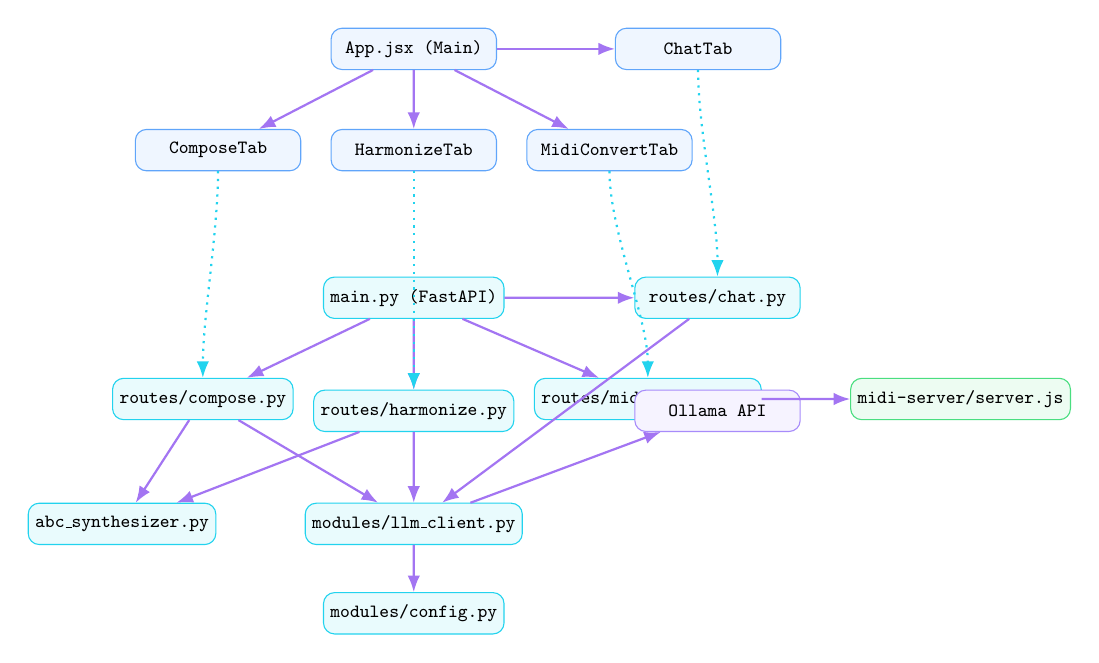
\begin{tikzpicture}[
    scale=0.75, every node/.style={transform shape},
    node distance=1.2cm and 1.5cm,
    % スタイル定義
    fe/.style={draw=node-ui, fill=node-ui!10, rounded corners=4pt, minimum width=2.8cm, minimum height=0.7cm, font=\small\ttfamily, align=center},
    be/.style={draw=node-api, fill=node-api!10, rounded corners=4pt, minimum width=2.8cm, minimum height=0.7cm, font=\small\ttfamily, align=center},
    ext/.style={draw=node-midi, fill=node-midi!10, rounded corners=4pt, minimum width=2.8cm, minimum height=0.7cm, font=\small\ttfamily, align=center},
    ol/.style={draw=node-ollama, fill=node-ollama!10, rounded corners=4pt, minimum width=2.8cm, minimum height=0.7cm, font=\small\ttfamily, align=center},
    dep/.style={-{Latex[length=6pt]}, thick, draw=brand-purple!70}
  ]

  % Frontend Nodes
  \node[fe] (app) {App.jsx (Main)};
  \node[fe, below left=1cm and 0.5cm of app] (comp) {ComposeTab};
  \node[fe, below=1cm of app] (harm) {HarmonizeTab};
  \node[fe, below right=1cm and 0.5cm of app] (midiconv) {MidiConvertTab};
  \node[fe, right=2cm of app] (chat) {ChatTab};

  \draw[dep] (app) -- (comp);
  \draw[dep] (app) -- (harm);
  \draw[dep] (app) -- (midiconv);
  \draw[dep] (app) -- (chat);

  % Backend Nodes (FastAPI)
  \node[be, below=3.5cm of app] (main) {main.py (FastAPI)};
  \node[be, below left=1cm and 0.5cm of main] (rcompose) {routes/compose.py};
  \node[be, below=1.2cm of main] (rharmonize) {routes/harmonize.py};
  \node[be, below right=1cm and 0.5cm of main] (rmidi) {routes/midi\_convert.py};
  \node[be, right=2.2cm of main] (rchat) {routes/chat.py};

  \draw[dep] (main) -- (rcompose);
  \draw[dep] (main) -- (rharmonize);
  \draw[dep] (main) -- (rmidi);
  \draw[dep] (main) -- (rchat);

  % Shared Backend modules
  \node[be, below=1.2cm of rharmonize] (llmclient) {modules/llm\_client.py};
  \node[be, left=1.5cm of llmclient] (synthesizer) {abc\_synthesizer.py};
  \node[be, below=0.8cm of llmclient] (config) {modules/config.py};
  
  \draw[dep] (rcompose) -- (llmclient);
  \draw[dep] (rharmonize) -- (llmclient);
  \draw[dep] (rchat) -- (llmclient);
  
  \draw[dep] (rcompose) -- (synthesizer);
  \draw[dep] (rharmonize) -- (synthesizer);
  \draw[dep] (llmclient) -- (config);

  % External Connectors
  \node[ext, right=1.5cm of rmidi] (node-srv) {midi-server/server.js};
  \node[ol, below=1.2cm of rchat] (ollama-api) {Ollama API};

  \draw[dep] (rmidi) -- (node-srv);
  \draw[dep] (llmclient) -- (ollama-api);

  % Frontend to Backend (HTTP Connectors)
  \draw[dep, dotted, brand-cyan] (comp.south) .. controls +(0,-1) and +(0,1) .. (rcompose.north);
  \draw[dep, dotted, brand-cyan] (harm.south) -- (rharmonize.north);
  \draw[dep, dotted, brand-cyan] (midiconv.south) .. controls +(0,-1) and +(0,1) .. (rmidi.north);
  \draw[dep, dotted, brand-cyan] (chat.south) .. controls +(0,-1) and +(0,1) .. (rchat.north);

\end{tikzpicture}
\caption{フロントエンド・バックエンドにおけるモジュール依存関係}
\label{fig:dependency}
\end{figure}

%===============================================================
% 08_license.tex - ライセンスと保証免責事項
%===============================================================
\section{ライセンスと品質保証・免責事項}

本章では、開発元（以下「メーカー」）が提供する本システム（ABC Music Suite）の利用条件、メーカーが負う責任範囲、および保証内容について規定します。本システムを使用することにより、利用者は本規定に同意したものとみなされます。

\subsection{製品保証とサポートの範囲}

本システムは、特定の開発・評価用プロトタイプとして設計されています。メーカーは、本システムが利用者の特定の目的に適合すること、または動作に中断やエラーが生じないことについて、明示的にも黙示的にも保証いたしません。

\subsubsection{1. 動作保証環境}
メーカーが動作を確認し、サポート対象とする基本環境は以下の通りです。これら以外の環境（独自のOSカスタム、サポート対象外のPythonバージョンなど）における不具合については、メーカーは対応いたしかねます。
\begin{itemize}
  \item \textbf{ホストPC}: Windows 10/11 (64bit), Python 3.10以上, Node.js 18以上
  \item \textbf{Ollama}: 推奨モデル \texttt{qwen3.5:9b} および \texttt{qwen2.5-coder:7b}
  \item \textbf{Raspberry Pi}: Raspberry Pi OS (Bullseye/Bookworm), Python 3.9以上, ALSA音響ユーティリティが正常にインストールされていること
\end{itemize}

\subsubsection{2. 生成物（音楽データおよびテキスト）に関する責任}
本システムで生成されるABC楽譜データおよびWAV音源は、すべてローカルLLM（AI）による推論の帰結です。
\begin{itemize}
  \item \textbf{出力の不確実性}: AIの性質上、常に音楽的に正しい結果が出力されるとは限りません。生成された楽譜における不協和音、音割れ、演奏不可能なフレーズの出現について、メーカーは修正の義務を負いません。
  \item \textbf{権利関係}: 生成された楽曲が第三者の著作権またはその他の権利を侵害しないことについて、メーカーは保証しません。生成物の商業利用や公開に際しては、利用者の自己責任において法的確認を行ってください。
\end{itemize}

\subsection{責任の制限（免責事項）}

本ソフトウェアの使用または使用不能から生じるすべての直接的、間接的、付随的、特別または結果的な損害（データの損失、業務の停止、ラズパイ等のハードウェア故障、ネットワーク帯域の枯渇、不正アクセス等を含む）について、メーカーおよび開発者は、契約上の請求、不法行為（過失を含む）、またはその他の法的根拠のいずれによるかを問わず、一切の責任を負いません。

\begin{tcolorbox}[warnbox, title=セキュリティに関するメーカーからの警告]
  ホストPC側で Ollama サーバーを外部公開設定（\texttt{OLLAMA\_HOST=0.0.0.0}）にする場合、同一LAN内のすべての機器からLLMサーバーへのアクセスが可能になります。
  公共のネットワーク（公衆Wi-Fiなど）でこの設定を行った場合、外部から不正に利用されたり、ホストPCに負荷をかけられたりする危険性があります。外部公開は必ず信頼できるプライベートなネットワーク内でのみ実行してください。この設定に起因する不正アクセスについて、メーカーは一切の責任を負いません。
\end{tcolorbox}

\subsection{ライセンス規定}

本システムのソースコードおよびドキュメントは、**MITライセンス**のもとで許諾されます。

\begin{tcolorbox}[mybox, title=MIT License]
\small
\ttfamily
Copyright (c) 2026 ABC Music Suite 開発チーム

Permission is hereby granted, free of charge, to any person obtaining a copy
of this software and associated documentation files (the "Software"), to deal
in the Software without restriction, including without limitation the rights
to use, copy, modify, merge, publish, distribute, sublicense, and/or sell
copies of the Software, and to permit persons to whom the Software is
furnished to do so, subject to the following conditions:

The above copyright notice and this permission notice shall be included in all
copies or substantial portions of the Software.

THE SOFTWARE IS PROVIDED "AS IS", WITHOUT WARRANTY OF ANY KIND, EXPRESS OR
IMPLIED, INCLUDING BUT NOT LIMITED TO THE WARRANTIES OF MERCHANTABILITY,
FITNESS FOR A PARTICULAR PURPOSE AND NONINFRINGEMENT. IN NO EVENT SHALL THE
AUTHORS OR COPYRIGHT HOLDERS BE LIABLE FOR ANY CLAIM, DAMAGES OR OTHER
LIABILITY, WHETHER IN AN ACTION OF CONTRACT, TORT OR OTHERWISE, ARISING FROM,
OUT OF OR IN CONNECTION WITH THE SOFTWARE OR THE USE OR OTHER DEALINGS IN THE
SOFTWARE.
\end{tcolorbox}


\end{document}
